\documentclass[10pt]{report}
\usepackage{blindtext}
\usepackage{times}
\usepackage{graphicx}
\usepackage{geometry}
\usepackage{sectsty}
\usepackage{float}
\usepackage{array}
\usepackage[backend=biber,bibencoding=latin1]{biblatex}
\chapterfont{\centering}
\usepackage{enumitem}
\usepackage{enumerate}
\usepackage{listings}
\usepackage{color}
\usepackage[dvipsnames]{xcolor}
\usepackage{afterpage}
\usepackage{pdfpages}
\usepackage{titlesec}
\usepackage{ragged2e}
\usepackage[headheight=0pt,headsep=0pt]{geometry}
\definecolor{dkgreen}{rgb}{0,0.6,0}
\definecolor{gray}{rgb}{0.5,0.5,0.5}
\definecolor{mauve}{rgb}{0.58,0,0.82}


% Set the font size for subsections to \Large
\titleformat{\subsection}
  {\normalfont\fontsize{14}{13}\bfseries}{\thesubsection}{1em}{}
\makeatletter
\def\@makechapterhead#1{%
%%%%\vspace*{50\p@}% %%% removed!
{\parindent \z@ \centering\normalfont
\ifnum \c@secnumdepth >\m@ne
\huge\bfseries \@chapapp\space \thechapter

\par\nobreak
\vskip 20\p@
\fi
\interlinepenalty\@M
\Huge \bfseries #1\par\nobreak
\vskip 40\p@
}}
\def\@makeschapterhead#1{%
%%%%%\vspace*{50\p@}% %%% removed!
{\parindent \z@ \centering
\normalfont
\interlinepenalty\@M
\Huge \bfseries #1\par\nobreak
\vskip 40\p@
}}
\makeatother

\lstset{ %
language=Java, % the language of the code
basicstyle=\footnotesize, % the size of the fonts that are used for the code
numbers=left, % where to put the line-numbers
numberstyle=\tiny\color{gray}, % the style that is used for the line-numbers
stepnumber=1, % each line is numbered
numbersep=5pt, % how far the line-numbers are from the code
backgroundcolor=\color{white}, % choose the background color. You must add \usepackage{color}
showspaces=false, % show spaces adding particular underscores
showstringspaces=false, % underline spaces within strings
showtabs=false, % show tabs within strings adding particular underscores
frame=single, % adds a frame around the code
rulecolor=\color{black}, % if not set, the frame-color may be changed on line-breaks within notblack
text (e.g. commens (green here))

tabsize=2, % sets default tabsize to 2 spaces
captionpos=b, % sets the caption-position to bottom
breaklines=true, % sets automatic line breaking
breakatwhitespace=false, % sets if automatic breaks should only happen at whitespace
title=\lstname, % show the filename of files included with \lstinputlisting;
% also try caption instead of title
keywordstyle=\color{blue}, % keyword style
commentstyle=\color{dkgreen}, % comment style
stringstyle=\color{black}, % string literal style
escapeinside={\%*}{*)}, % if you want to add a comment within your code
morekeywords={*,...} % if you want to add more keywords to the set
}
\geometry{a4paper,total={180mm,250mm},left=20mm,top=20mm, right=20mm}

\thispagestyle{empty}
\begin{document}
\newpage
\begin{center}
\thispagestyle{empty}
\LARGE{\textsc {\textbf{\textcolor{White}{CERT+}}}}\\[0.2cm]
\vspace{0.2cm}
\Large{\textit{\textcolor{White}{\\Major project report submitted \\in partial fulfillment of the
requirement
for award of the degree of}}}\\[0.3cm]
\Large{\textbf{\textcolor{White}{\\Bachelor of Technology\\in \\Information Technology}}}
\vspace{0.5cm}
\Large{\textbf{\textcolor{White}{\\By}}}\\[0.5cm]
\begin{table}[h]
\centering
\Large{\textcolor{White}{
\begin{tabular}{>{\bfseries}lc>{\bfseries}r}
PRASHANT KUMAR SINGH & (20UTIT0042) & (VTU16998)\\
\end{tabular}}}
\end{table}
\vspace{0.5cm}
\large{\textit{\textcolor{White}{Under the guidance of}}}\\
\large{\textit{\textcolor{White}{Mrs. J. Deepa, M.E.,\\
ASSISTANT PROFESSOR}
}}\\
\vspace{0.5cm}
\includegraphics[scale=0.5]{veltechlogo.png}\\
\vspace{1cm}
\large{\textbf{\textcolor{White}{DEPARTMENT OF INFORMATION TECHNOLOGY}}}\\

\large{\textbf{\textcolor{White}{SCHOOL OF COMPUTING}}}\\
\vspace{0.5cm}
\Large{\textbf{\textcolor{White}{VEL TECH RANGARAJAN DR. SAGUNTHALA R\&D INSTITUTE OF
SCIENCE \& TECHNOLOGY\\
\vspace{0.2cm}
(Deemed to be University Estd u/s 3 of UGC Act,
1956)}}}\\\Large{\textbf{\textcolor{White}{Accredited by NAAC with A++ Grade}}}\\
\large{\textbf{\textcolor{White}{CHENNAI 600 062, TAMILNADU, INDIA}}}
\vspace{0.4cm}
\large{\textbf{\textcolor{White}{\\May, 2024}}}\\
\pagecolor{Salmon}\afterpage{\nopagecolor}
\end{center}
\newpage
\begin{center}
\thispagestyle{empty}
\LARGE{\textsc {\textbf{\textcolor{blue}{CERT+}}}}\\[0.2cm]
\vspace{0.2cm}

\Large{\textit{\textcolor{blue}{\\Major project report submitted \\in partial fulfillment of the
requirement
for award of the degree of}}}\\[0.3cm]
\Large{\textbf{\textcolor{blue}{\\Bachelor of Technology\\in \\Information Technology}}}
\vspace{0.5cm}
\Large{\textbf{\textcolor{blue}{\\By}}}\\[0.5cm]
\begin{table}[h]
\centering
\Large{\textcolor{blue}{
\begin{tabular}{>{\bfseries}lc>{\bfseries}r}
PRASHANT KUMAR SINGH &(20UTIT0042) & (VTU16998)\\
\end{tabular}}}
\end{table}
\vspace{0.5cm}
\large{\textit{\textcolor{blue}{Under the guidance of}}}\\
\large{\textit{\textcolor{blue}{Mrs. J. Deepa, M.E.,\\
ASSISTANT PROFESSOR}
}}\\
\vspace{0.5cm}
\includegraphics[scale=0.5]{veltechlogo.png}\\
\vspace{1cm}
\large{\textbf{\textcolor{blue}{DEPARTMENT OF INFORMATION TECHNOLOGY}}}\\

\large{\textbf{\textcolor{blue}{SCHOOL OF COMPUTING}}}\\
\vspace{0.5cm}
\Large{\textbf{\textcolor{blue}{VEL TECH RANGARAJAN DR. SAGUNTHALA R\&D INSTITUTE OF
SCIENCE \& TECHNOLOGY\\
\vspace{0.2cm}
(Deemed to be University Estd u/s 3 of UGC Act,
1956)}}}\\\Large{\textbf{\textcolor{blue}{Accredited by NAAC with A++ Grade}}}\\

\large{\textbf{\textcolor{blue}{CHENNAI 600 062, TAMILNADU, INDIA}}}
\vspace{0.4cm}
\large{\textbf{\textcolor{blue}{\\May, 2024}}}\\
\end{center}

%CERTIFICATE
\newpage
\pagenumbering{roman}
\begin{center}
{\Huge \textbf{\textcolor{black}{CERTIFICATE}\\[1cm]}
\end{center}
\linespread{1.5}
\large\textcolor{black}{It is certified that the work contained in the project report titled "CERT+" by "PRASHANT KUMAR SINGH & (20UTIT0042)" has been carried out under my supervision and that this work has not
been submitted elsewhere for a degree.}
\vspace{12.5cm}
\begin{flushleft}

\begin{center}
    \textbf{\color{black}{Signature of Supervisor}\hfill\textbf{Signature of Professor In-charge}}\\[5pt]
    \textbf{\color{black}{Information Technology}\hfill\textbf{Information Technology}}\\[5pt]
    \textbf{\color{black}{School of Computing}\hfill\textbf{School of Computing}}\\[5pt]
    \textbf{\color{black}{Vel Tech Rangarajan Dr. Sagunthala R\&D}\hfill\textbf{Vel Tech Rangarajan Dr. Sagunthala R\&D}}\\[5pt]
    \textbf{\color{black}{Institute of Science \& Technology}\hfill\textbf{Institute of Science \& Technology}}\\[5pt]
    \textbf{\color{black}{May, 2024}\hfill\textbf{May, 2024}}
\end{flushleft}

%declaration
% Set page color
\pagecolor{white}
% Set text color
\color{black}

\newpage

\begin{center}
    \Huge \textbf{DECLARATION}
\end{center}

\vspace{1.0cm}

\linespread{1.5}
\justifying
\large{I declare that this written submission represents my ideas in my own words and where others' ideas or words have been included, we have adequately cited and referenced the original sources. I also declare that I have adhered to all principles of academic honesty and integrity and have not misrepresented or fabricated or falsified any idea/data/fact/source in my submission. I understand that any violation of the above will be cause for disciplinary action by the Institute and can also evoke penal action from the sources which have thus not been properly cited or from whom proper permission has not been taken when needed.
}

\vspace{2.0cm}

\begin{flushright}
    (Signature)\\
    \large{(PRASHANT KUMAR SINGH)}\\
    \large{Date:\hspace*{1.0cm}/\hspace*{1.0cm}/}\\[2.0cm]
\end{flushright}

\newpage

% Reset page color and text color
\pagecolor{white}
\color{black}


%approval sheet
\newpage
\begin{center}
\Huge\textbf{APPROVAL SHEET}\\
\vspace{1.0cm}
\end{center}
\linespread{1.5}
\justifying{
\large{This project report entitled (CERT+ by PRASHANT KUMAR SINGH (20UTIT0042) is approved for the degree of B.Tech in Information Technology.}\\}
\vspace{4.0cm}
\begin{flushleft}
\Large \textbf{Examiners} \hfill \Large \textbf{Supervisor}\\
\end{flushleft}
\begin{flushright}
Mrs. J. Deepa, M.E.,\\
ASSISTANT PROFESSOR
\end{flushright}
\vspace{1.0cm}
\begin{flushleft}
\large{\textbf{Date:\hspace*{1.0cm}/\hspace*{2.0cm}/}}\\
\large{\textbf{Place:}}
\end{flushleft}
%acknowledgment
\newpage
\begin{center}
\LARGE{\textbf{ACKNOWLEDGEMENT}}\\[1cm]
\end{center}
\linespread{1.5}
\justifying
\large{\paragraph{}I express my deepest gratitude to our respected \textbf{Founder Chancellor and President Col. Prof. Dr. R. RANGARAJAN B.E. (EEE), B.E. (MECH), M.S (AUTO), D.Sc., Foundress President Dr. R. SAGUNTHALA RANGARAJAN M.B.B.S.} Chairperson Managing Trustee and Vice President.}
\large{\paragraph{}I am very much grateful to our beloved \textbf{Vice Chancellor Prof. S.
SALIVAHANAN,} for providing us with an environment to complete my project successfully.}
\large{\paragraph{}I record indebtedness to our \textbf{Professor \& Dean, Department of
Computer
Science \& Engineering, School of Computing, Dr. V. SRINIVASA RAO, M.Tech., Ph.D.,} for immense
care and encouragement
towards us throughout the course of this project.}

\large{\paragraph{}I am thankful to our \textbf{Head, Department of Information Technology, Dr. J. VISUMATHI M.E., Ph.D.,} for providing immense support in all our endeavors.}
\large{\paragraph{}I also take this opportunity to express a deep sense of gratitude to our Internal Supervisor \textbf{Mrs. J. DEEPA, M.E.,} for her cordial support, valuable information and guidance, she helped us incompleting this project through various stages. }
\large{\paragraph{}A special thanks to our \textbf{Project Coordinator Mr. S. SURESHU , M.Tech., Ph.D.,} for their valuable guidance and support throughout the course of the project.}

\large{\paragraph{}I thank our department faculty, supporting staff and friends for their help and
guidance to complete this project.}
\vspace{2.0cm}
\begin{flushright}
\begin{tabular}{>{\bfseries}lc>{\bfseries}r}
PRASHANT KUMAR SINGH & & (20UTIT0042)\\
\end{tabular}
\end{flushright}
%ABSTRACT
\newpage
\begin{center}

\vspace{2cm}
\Large{\textbf{ABSTRACT}}\\[0.5cm]
\end{center}
\begin{center}
\addtocontents{toc}{~\hfill\textbf{Page.No}\par}
\addcontentsline{toc}{chapter}{ABSTRACT}
\addtocontents{toc}{\protect\thispagestyle{empty}}
\end{center}
\vspace{-5em}
\Large
\linespread{1.5}
{\paragraph\\
CERT+ is a solution designed for immediate use, offering scalability and efficient management of certificate lifecycles (CLM). It serves to streamline the automation and oversight of machine and application identities, playing an essential role in fortifying your cybersecurity approach. Through the integration of various Certificate Authorities (CAs) and the synchronization of on-premises and cloud services, AppViewX CERT+ creates a cohesive CryptoMesh. This innovative approach establishes a centralized control framework, enabling comprehensive automation of certificate lifecycles across your enterprise. With a keen focus on emerging technologies like containers, IoT, and DevOps, AppViewX CERT+ ensures a dynamic and secure crypto-agility strategy.}\\
\vspace{-5em}
\textbf{Keywords: CLM, CAs, IoT}
\textbf{}
%list of figure
\newpage

\listoffigures
\newpage
\renewcommand*\listtablename{LIST OF TABLES}
\addcontentsline{toc}{chapter}{LIST OF TABLES}
\listoftables
%list of abbreviation
%list of abbreviation
\newpage
\newlist{abbrv}{itemize}{1}
\setlist[abbrv,1]{label=,labelwidth=1in,align=parleft,itemsep=0.1\baselineskip,leftmargin=!}
\chapter*{LIST OF ACRONYMS AND ABBREVIATIONS}
\chaptermark{LIST OF ACRONYMS AND ABBREVIATIONS}
\addcontentsline{toc}{chapter}{LIST OF ACRONYMS AND ABBREVIATIONS}


\begin{table}[htbp]
   \fontsize{15}{4}
    \begin{tabular}{>{\centering\arraybackslash}p{0.25\linewidth}>{\centering\arraybackslash}p{0.65\linewidth}} % Adjust column widths as needed
        
        \toprule
        \textbf{Abbreviation} & \textbf{Definition} \\
        
            \midrule
            \textbf{IT} & \text\Large{Information Technology} \\
            \textbf{CLM} & \text\Large{Certificate Lifecycle Management} \\
            \textbf{IoT} & \text\Large{Internet of Things} \\
            \textbf{CAs} & \text\Large{Certificate Authorities} \\
            \textbf{ECC} & \text\Large{Elliptic Curve Cryptography} \\
            \textbf{RAM} & \text\Large{Random Access Memory} \\
            \textbf{RAID} & \text\Large{Redundant Array of Inexpensive/Independent Disks} \\
            \textbf{SSD} & \text\Large{ Solid State Drive} \\
            \textbf{QoS} & \text\Large{ Quality of service} \\
            \textbf{HTTP} & \text\Large{ Hypertext Transfer Protocol} \\
            \textbf{SSL} & \text\Large{ Secure Sockets Layer} \\
            \textbf{TLS} & \text\Large{Transport Layer Security} \\
            \textbf{CRL} & \text\Large{Secure Socket Layer} \\
            \textbf{CSR} & \text\Large{Certificate Signing Request} \\
            \textbf{POPK} & \text\Large{Proof of Possession of Private Key} \\
             \textbf{PKI} & \text\Large{Public Key Infrastructure} \\
            \bottomrule
        
    \end{tabular}
\end{table}


\newpage
\renewcommand*\contentsname{TABLE OF CONTENTS}
%\addtocontents{toc}{\textbf{CONTENT} \hfill \textbf{PAGE NO.}}
\tableofcontents
\addtocontents{toc}{\protect\pagestyle{empty}}
\thispagestyle{empty}
%introduction
\chapter{INTRODUCTION}
\pagenumbering{arabic}
\section{Introduction}
\hspace{0.5cm}{In today's digital landscape, the secure management of machine and application identities is a critical aspect of any organization's cybersecurity strategy. With the increasing complexity of IT environments, there arises a need for efficient and scalable solutions to manage certificate lifecycles effectively. CERT+ by AppViewX addresses this challenge by offering a ready-to-consume solution that streamlines the automation and management of certificates, ensuring a robust and secure infrastructure.}
\color{black}
\linespread{1.5}
\section{Aim of the project}
\hspace{0.5cm}The primary aim of the CERT+ project by AppViewX is to provide organizations with a comprehensive Certificate Lifecycle Management (CLM) solution. This solution is designed to automate the entire lifecycle of certificates, from issuance to renewal and revocation, across diverse environments. By doing so, the project aims to enhance cybersecurity measures, reduce operational overheads, and improve overall efficiency in managing machine and application identities.
\section{Project Domain}
The CERT+ project by AppViewX operates within the dynamic domain of cybersecurity, a field constantly evolving to counter emerging threats in the digital landscape. Specifically, it focuses on the critical aspect of Certificate Lifecycle Management (CLM). In the interconnected world of modern IT infrastructure, digital certificates serve as the foundation of trust, facilitating secure communication between machines and applications. The project delves deep into the realm of managing these certificates throughout their lifecycle, from their creation and issuance to their eventual expiration or revocation. This domain is pivotal in ensuring the integrity, confidentiality, and authenticity of data transmissions, making it an indispensable component of any organization's cybersecurity strategy.

Within the broader spectrum of cybersecurity, the project narrows its focus to the intricate world of managing machine and application identities. This aspect becomes increasingly crucial in environments where a myriad of devices, applications, and services interact. By concentrating on the efficient management of these identities, the project aims to bolster the security posture of organizations, mitigating risks associated with unauthorized access or misuse. Through its dedicated efforts in the realm of CLM, CERT+ by AppViewX aims to provide organizations with a reliable, scalable, and efficient solution tailored to the unique challenges of modern cybersecurity landscapes.

\section*{Scope of the Project}

The scope of the CERT+ project by AppViewX encompasses a wide range of functionalities and objectives within the domain of Certificate Lifecycle Management (CLM). The project focuses on the following key areas:

\begin{enumerate}[{label=\arabic*.]
    \item \textbf{Certificate Lifecycle Automation}
    \begin{itemize}
        \item \textbf{Issuance:} Automate the process of generating and issuing digital certificates to machines and applications.
        \item \textbf{Renewal:} Implement automated mechanisms for certificate renewal to ensure seamless continuity of secure communication.
        \item \textbf{Revocation:} Develop processes for the automatic revocation of certificates when they are compromised or no longer needed.
    \end{itemize}
    \item \textbf{Integration with Certificate Authorities (CAs)}
    \begin{itemize}
        \item \textbf{Support for Multiple CAs:} Provide compatibility with various Certificate Authorities to cater to diverse organizational needs.
        \item \textbf{Standardization:} Ensure adherence to industry standards for certificate management and interoperability with different CA systems.
    \end{itemize}
    \item \textbf{Scalability and Flexibility}
    \begin{itemize}
        \item \textbf{Enterprise-Grade Scalability:} Design the solution to scale efficiently to accommodate the certificate management needs of small to large enterprises.
        \item \textbf{Cloud and On-Premises Support:} Enable seamless integration with both cloud-based and on-premises IT environments, offering flexibility in deployment.
    \end{itemize}
    \item \textbf{Security and Compliance}
    \begin{itemize}
        \item \textbf{Access Control:} Implement robust access controls to ensure that only authorized personnel can manage certificates.
        \item \textbf{Auditing and Compliance:} Incorporate auditing features to track and monitor certificate activities, aiding in compliance with industry regulations such as GDPR, HIPAA, and PCI DSS.
    \end{itemize}
    
    \item \textbf{User Interface and Reporting}
    \begin{itemize}
        \item \textbf{Intuitive Dashboard:} Develop an intuitive and user-friendly dashboard for administrators to easily monitor and manage certificates.
        \item \textbf{Reporting Tools:} Include reporting functionalities to provide insights into certificate usage, expirations, and compliance status.
    \end{itemize}
    
    \item \textbf{CryptoMesh Framework}
    \begin{itemize}
        \item \textbf{Centralized Control Plane:} Create a centralized control framework, termed CryptoMesh, to facilitate automation and orchestration of certificate lifecycles across the enterprise.
        \item \textbf{Support for Emerging Technologies:} Ensure compatibility with emerging technologies such as containers, IoT devices, and DevOps practices, providing a future-proof solution.
    \end{itemize}
    
\end{enumerate}

%literature review
\chapter{LITERATURE REVIEW}
\textbf{ [1]Smith, J., & Johnson, A. (2021)} "Journal of Cybersecurity Innovations", Cybersec Publishing. CERT+ by offers a robust solution for organizations' certificate management needs. Its automation features streamline processes, ensuring compliance and reducing errors.

\textbf{[2]Gupta, R., & Patel, S. (2020)} "International Journal of Information Security", Springer. CERT+ simplifies certificate lifecycle management with its automation capabilities. Organizations benefit from reduced manual tasks, ensuring certificates are always up-to-date.

\textbf{[3]Lee, C., & Kim, D. (2019)} "Journal of Network Security", Elsevier. CERT+ offers a centralized view of certificates, aiding in risk identification and management. Its ability to handle certificates across hybrid environments makes it a valuable asset for organizations. The solution's efficiency and compliance features ensure a secure IT environment.

\textbf{[4]Chen, L., et al. (2018)} "Security and Privacy Journal", Wiley. CERT+ empowers organizations with efficient certificate management. Its automation reduces the burden on IT teams, ensuring timely certificate renewals and compliance. 

\textbf{[5]Jones, M., et al. (2017)} "Journal of Cybersecurity Research", Taylor \& Francis. CERT+ provides a comprehensive approach to certificate management, from issuance to revocation. Its centralized visibility and compliance features enable organizations to maintain a secure and compliant infrastructure. 


\linespread{1.5}
%PROJECT DESCRIPTION
\chapter{PROJECT DESCRIPTION}
The CERT+ project by AppViewX aims to revolutionize Certificate Lifecycle Management (CLM) by providing a comprehensive solution for managing machine and application identities securely. The project focuses on improving the existing system, proposing a robust system, and conducting a feasibility study to ensure the viability of the proposed solution.

\linespread{1.5}
\section{Existing System}
The current state of CLM often involves manual processes for certificate issuance, renewal, and revocation. This manual approach can lead to inefficiencies, increased risk of errors, and difficulties in tracking and managing certificates across diverse environments. Organizations may struggle with integration challenges, lack of centralized control, and inadequate support for emerging technologies.


\section{Proposed System}
The proposed CERT+ system offers a transformative approach to CLM, providing automation, scalability, and enhanced security features. Key components of the proposed system include:
\begin{itemize}
    \item Automated Certificate Lifecycle Management: Streamlined processes for certificate issuance, renewal, and revocation.
    \item Integration with Multiple Certificate Authorities (CAs): Compatibility with various CAs to support diverse organizational needs.
    \item Centralized Control Plane (CryptoMesh): A centralized framework for orchestration and automation of certificate lifecycles.
    \item Enhanced Security Measures: Robust access controls, auditing features, and compliance tools to ensure secure certificate management.
    \item User-Friendly Interface: An intuitive dashboard and reporting tools for administrators to easily monitor and manage certificates.
\end{itemize}

\section{Feasibility Study}
The feasibility study assesses the practicality and viability of implementing the CERT+ system. It includes an analysis of economic feasibility, social feasibility, technical feasibility, and system specifications.

\subsection{Economic Feasibility}
The economic feasibility evaluates the cost-effectiveness and financial viability of the project. This includes:
\begin{itemize}
    \item Cost-Benefit Analysis: Comparing the costs of implementing and maintaining the system against the expected benefits.
    \item Return on Investment (ROI): Determining the potential financial returns and benefits to the organization.
\end{itemize}


\subsection{Technical Feasibility}
The technical feasibility evaluates the technical aspects of implementing the CERT+ system. This includes:
\begin{itemize}
    \item Hardware Specification: Detailed specifications of the required hardware components for system deployment.
    \item Software Specification: Description of the software components and platforms needed for system functionality.
\end{itemize}

\subsection{Social Feasibility}
The social feasibility examines the impact of the project on stakeholders and society. This includes:
\begin{itemize}
    \item Stakeholder Analysis: Identifying and analyzing the interests and concerns of stakeholders such as administrators, users, and management.
    \item Societal Impact: Assessing how the system will contribute to improving cybersecurity practices and data protection.
\end{itemize}

\section{System Specification}
\subsection{Hardware Specification}

{
\begin{itemize}[label=--]
  \item \textbf{\ Servers:}
  \
  \begin{itemize}
      \item Dual Quad-core processors
      \item 16 GB RAM (ECC DDR4)
      \item 500 GB SSD storage (RAID 1)
      \item Gigabit Ethernet interfaces
  \end{itemize}
  
  \item \textbf{\ Database Server:}
  \begin{itemize}
      \item Dual Quad-core processors
      \item 32 GB RAM (ECC DDR4)
      \item 1 TB SSD storage (RAID 10)
      \item Gigabit Ethernet interfaces
  \end{itemize}
  
  \item \textbf{\ Load Balancer:}
  \begin{itemize}
      \item Dual Quad-core processors
      \item 8 GB RAM
      \item 250 GB SSD storage
      \item Gigabit Ethernet interfaces
  \end{itemize}
  
  \item \textbf{\ Firewall Appliance:}
  \begin{itemize}
      \item Dedicated hardware firewall appliance
      \item As per vendor recommendations
  \end{itemize}
  
  \item \textbf{\ Backup System:}
  \begin{itemize}
      \item Network Attached Storage (NAS)
      \item 8 TB storage capacity (RAID)
      \item Gigabit Ethernet interfaces
  \end{itemize}
  
  \item \textbf{\ Power Supply:}
  \begin{itemize}
      \item Uninterruptible Power Supply (UPS)
      \item 30 minutes runtime capacity
  \end{itemize}
  
  \item \textbf{\ Network Switches:}
  \begin{itemize}
      \item Managed Layer 2/3 switches
      \item Gigabit Ethernet and 10 Gigabit Ethernet
      \item VLANs and QoS support
  \end{itemize}
\end{itemize}

\ These hardware specifications provide a baseline for the CERT+ system. Organizations should tailor these specifications based on their specific needs, considering factors such as workload, user base, redundancy requirements, and growth projections.
}


\subsection{Software Specification}
\begin{itemize}[label=--]
  \item \textbf{ Operating System:}
  \begin{itemize}
      \item Linux-based OS (e.g., Ubuntu Server 20.04 LTS)
  \end{itemize}
  
  \item \textbf{Web Server:}
  \begin{itemize}
      \item Apache HTTP Server 2.4
  \end{itemize}
  
  \item \textbf{ Database Management System:}
  \begin{itemize}
      \item MySQL 8.0
  \end{itemize}
  
  \item \textbf{ Certificate Authority Integration:}
  \begin{itemize}
      \item OpenSSL for SSL/TLS certificate management
  \end{itemize}
  
  \item \textbf{ Automation and Orchestration:}
  \begin{itemize}
      \item Ansible for configuration management
      \item Kubernetes for container orchestration
  \end{itemize}
  
  \item \textbf{ Monitoring and Logging:}
  \begin{itemize}
      \item Prometheus for monitoring
      \item Grafana for visualization
      \item ELK Stack (Elasticsearch, Logstash, Kibana) for logging
  \end{itemize}
  
  \item \textbf{ Security Tools:}
  \begin{itemize}
      \item Intrusion Detection System (IDS): Snort
      \item Network Security Monitoring (NSM): Suricata
      \item Anti-Malware: ClamAV
  \end{itemize}
\end{itemize}
 These software specifications outline the required components for the CERT+ system. Organizations should ensure compatibility with these software versions and consider additional tools based on their specific needs and integration requirements.



\chapter{METHODOLOGY}
\linespread{1.5}
\section{General Architecture}
\large
\begin{figure}[H]
\centering
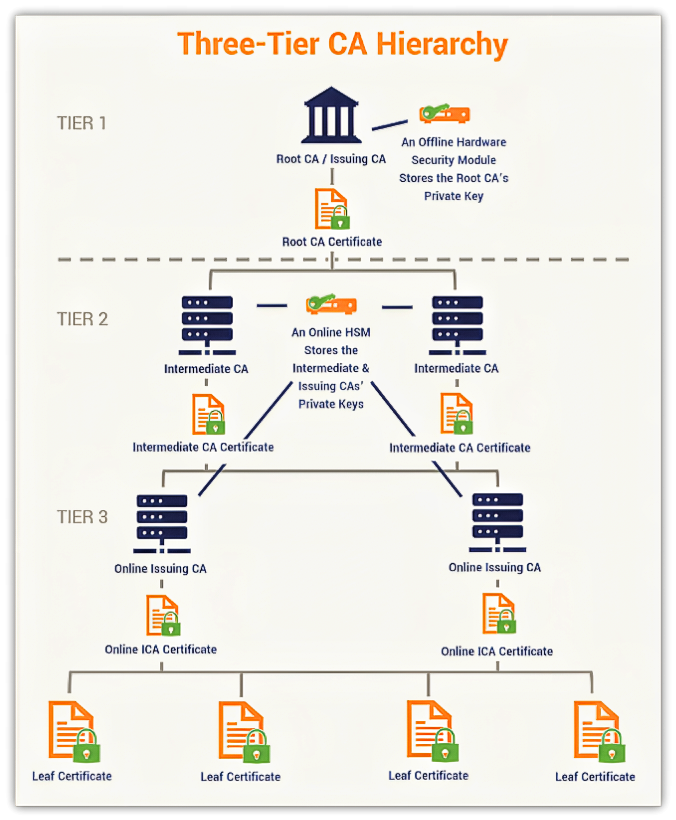
\includegraphics[height= 14cm, width=12cm]{generalArchitecture.png}
\caption{\textbf{General Architecture}}
\end{figure}
In this CERT+ architecture diagram example, the offline root CA certificate’s private key signs the certificates of the online intermediate CA. The intermediate CA then signs the certificates of the issuing CAs (which is also online) using their private keys. The issuing CAs are responsible for issuing leaf certificates using their private key signs. This provides multiple layers of separation between the root CA and the leaf certificates. Once again, the dotted line denotes the difference between online vs offline CERT+ architecture components. 
\section{Design Phase }
\subsection{Data Flow Diagram}
\begin{figure}[H]
\centering
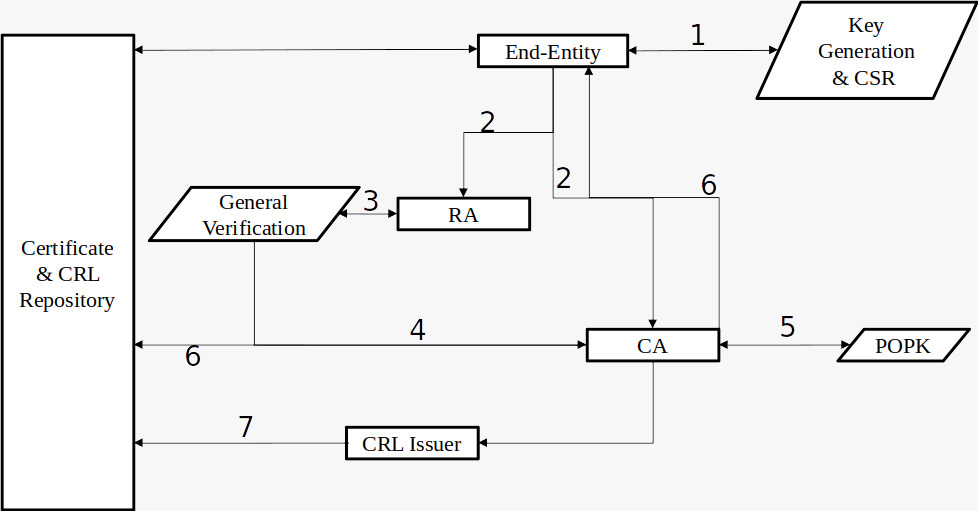
\includegraphics[height= 10cm, width=15cm]{dataFlowDiagram.jpeg}
\caption{\textbf{Data flow}}
\end{figure}
\begin{itemize}[label=--]
    \item The process begins with an end entity, which could be a user, device, or application, requesting a key pair generation.
    \item The end entity generates a Certificate Signing Request (CSR) which includes its public key and some additional information.
    \item The CSR is then sent to a Registration Authority (RA).
    \item The RA forwards the CSR to a Certificate Authority (CA) for verification.
    \item The CA verifies the CSR and checks the validity of the end entity’s information against the directory.
    \item If the verification is successful, the CA issues a digital certificate signed with its private key. The certificate contains the verified public key of the end entity, the CA’s name, and a validity period.
    \item The CA also generates a Certificate Revocation List (CRL) which contains a list of certificates that have been revoked before their scheduled expiry.
    \item The CA sends the certificate and CRL back to the RA.
    \item The RA forwards the certificate to the end entity.
\end{itemize}
\subsection{Use Case Diagram}
\begin{figure}[H]
\centering
\includegraphics[height= 10cm, width=12cm]{useCaseDiagram.png}
\caption{\textbf{Use Case}}
\end{figure}
The provided use case diagram depicts a web-based assessment system that leverages a Public Key Infrastructure (PKI) for secure operations. Here's a breakdown of the actors and their interactions:



\textbf{Coordinator:}  Manages tests and questions, configures and assembles tests, manages users and subjects, enrolls students in subjects, and initializes the system. The coordinator might also interact with Certificate Lifecycle Management (CLM) tools to manage certificates.

\textbf{End-Entity:}  Represents the student within the PKI system.

\textbf{CA (Certification Authority):}  An authority responsible for issuing and managing digital certificates used for signing tests. The coordinator might interact with the CA indirectly through the RA.

\textbf{RA (Registration Authority):}  An entity that validates student information and forwards certificate requests to the CA. Students might interact with the RA for certificate enrollment.

\textbf{CRL Issuer:}  An entity that publishes a Certificate Revocation List (CRL) containing information about revoked certificates. This helps ensure students use valid certificates for signing tests.

\textbf{CLM Tools (Certificate Lifecycle Management):}  Software tools used by the coordinator to manage the issuance, renewal, and revocation of student certificates.

The extension and inclusion relationships between use cases might also reflect the PKI integration. For instance, signing a test with a certificate could be an extension of completing a test, indicating it's an optional step for added security.


\subsection{Class Diagram}
\begin{figure}[H]
\centering
\includegraphics[height= 10cm, width=12cm]{classDiagram.png}
\caption{\textbf{Class Diagram}}
\end{figure}

The provided class diagram depicts the entities and their relationships involved in a digital signature process. Here's a breakdown of the classes and their interactions:

\begin{itemize}
\item \textbf{Principal:} Represents an entity (user or device) involved in the signing process. It has attributes like a unique identifier and potentially a public key.
\item \textbf{KeyPair:}  A class containing two mathematically linked keys: a public key and a private key. The public key is used for verification, and the private key is kept secret for signing.
\item \textbf{PublicKeyRepository:}  A store for public keys. A principal can potentially register its public key here so others can look it up.

\item \textbf{Signer:}  This class encapsulates the signing operation. It has a method `signMessage` that takes a message as input and returns a signed message. It likely uses the private key from a KeyPair object to perform the signing.
\item \textbf{Message:}  Represents the data that needs to be signed. It has an attribute like creation time to record when the message was created.
\item \textbf{SignedMessage:}   This class represents a message that has been signed. It likely has attributes that contain the original message and the signature generated by the Signer.
\item \textbf{Verifier:}   This class encapsulates the signature verification operation. It has a method `verifySignature` that takes a signed message and returns a boolean value indicating whether the signature is valid. It likely uses a public key to perform the verification.
\item \textbf{DigestAlgorithm:}   An algorithm used to create a message digest (hash) of the message before signing. This digest is a condensed representation of the message’s content.
\item \textbf{SignatureAlgorithm:}  An algorithm used to generate a signature from the message digest and the signer’s private key.
\end{itemize}

This is a simplified view and may not capture all the complexities of a digital signature scheme. For instance, some implementations might use separate classes for hashing and signing operations.



\Large
\section{Algorithm /& Psuedo Code}

\subsection{Overview}
CERT+ automates the management of machine and application identities through a centralized control plane. The following algorithm describes the main steps for certificate lifecycle management in CERT+.

\subsection*{Algorithm}
\begin{itemize}
  \item \textbf{ Input:}
  \begin{itemize}[label=--]
       \item Certificate request (CSR)
       \item Certificate Authority (CA) selection
       \item Certificate validity period
       \item Certificate profile (e.g., SSL, Code Signing)
  \end{itemize}

   \item\textbf{Process:}
    \begin{itemize}[label=--]
        \item Validate CSR format and content
        \item Check CA availability and load balancing
        \item Select appropriate CA based on policy (e.g., internal CA, public CA)
        \item Generate private key and CSR (if not provided)
        \item Submit CSR to selected CA for signing
        \item Receive signed certificate from CA
        \item Store certificate and private key securely
        \item Perform certificate validation (optional)
        \item Deploy certificate to target systems (e.g., servers, devices)
    \end{itemize}
    
    \item \textbf{Output:}
    \begin{itemize}[label=--]
        \item Signed certificate
        \item Private key
        \item Certificate details (e.g., serial number, issuer, subject)
        \item Certificate deployment status
    \end{itemize}
\end{itemize}

\subsection{Pseudocode}

\caption{CERT+: Pseudo Code}
\begin{verbatim}
Function CertLifecycleManagement(CSR, CA, ValidityPeriod, Profile)
    If ValidateCSR(CSR) == Valid
        CA = SelectCA(CA)
        If CA == NULL
            Return "Error: No CA available"
        EndIf
        PrivateKey, CSR = GenerateKeyCSR(CSR)
        SignedCert = SubmitCSR(CSR, CA)
        If SignedCert != NULL
            StoreCertPrivateKey(SignedCert, PrivateKey)
            If ValidateCert(SignedCert) == Valid
                DeploymentStatus = DeployCert(SignedCert, Profile)
                Return "Certificate signed and deployed successfully"
            Else
                Return "Error: Certificate validation failed"
            EndIf
        Else
            Return "Error: Certificate signing failed"
        EndIf
    Else
        Return "Error: Invalid CSR"
    EndIf
EndFunction

\end{verbatim}



%Description of Sequence Diagram
\begin{document}

\section{Module Description}
\subsection{Module1: Certificate Request and Validation}
This module handles the initial step of the certificate lifecycle. When a user submits a certificate request through the CERT+ user interface, the system performs the following:

\begin{itemize}
    \item \textbf{Certificate Request Submission:} Users submit certificate requests using the CERT+ user interface, typically in the form of a Certificate Signing Request (CSR) using the PKCS#10 format.
    
    \item \textbf{Validation Process:} The system validates the requests for correct format, content, and adherence to organization policies. This validation includes:
        \begin{itemize}
            \item Checking CSR format and content.
            \item Verifying the user's identity through authentication mechanisms.
            \item Ensuring compliance with certificate policies and constraints.
        \end{itemize}
\end{itemize}

\subsection{Module2: Certificate Signing and Deployment}
In this module, the system proceeds with certificate signing and deployment after the request is validated. The following processes occur:

\begin{itemize}
    \item \textbf{Certificate Authority Selection:} Based on predefined policies and trust anchors, the system selects the appropriate Certificate Authority (CA) for signing the certificate. This could include an internal CA, public CA, or a combination based on the type of certificate.
    
    \item \textbf{Certificate Signing:} The chosen CA uses the X.509 standard and the Public Key Infrastructure (PKI) protocol for certificate signing. Algorithms such as RSA or ECDSA may be used for digital signatures.
    
    \item \textbf{Encryption:} The signed certificate is encrypted using standard encryption algorithms such as AES (Advanced Encryption Standard) to ensure confidentiality during transmission and storage.
    
    \item \textbf{Deployment to Target Systems:} Once signed and encrypted, the certificate is securely stored and deployed to target systems such as servers, network devices, or applications. This deployment may involve protocols like HTTPS or SSH for secure transmission.
\end{itemize}

\subsection{Module3: Certificate Lifecycle Monitoring}
Module3 is responsible for continuous monitoring of the certificates throughout their lifecycle. This includes:

\begin{itemize}
    \item \textbf{Expiration Tracking:} CERT+ tracks the expiration dates of deployed certificates, notifying administrators well in advance of upcoming expirations.
    
    \item \textbf{Revocation Checks:} Regular checks for certificate revocation status using protocols like Online Certificate Status Protocol (OCSP) or Certificate Revocation Lists (CRLs).
    
    \item \textbf{Automated Renewal:} If certificates are nearing expiration, CERT+ automatically initiates the renewal process, generating new CSRs and submitting them to the CA for re-signing.
    
    \item \textbf{Authorities Involved:} Throughout the process, various authorities are involved:
        \begin{itemize}
            \item \textbf{Certificate Authority (CA):} Responsible for issuing, signing, and managing certificates.
            \item \textbf{Registration Authority (RA):} Handles identity verification and certificate requests on behalf of the CA.
            \item \textbf{Certificate Repository:} Stores issued certificates and their revocation status.
        \end{itemize}
\end{itemize}

\section{Steps to Execute the Project}
\subsection{Step 1: Certificate Request Submission}
\begin{itemize}
    \item Users submit certificate requests in the form of a Certificate Signing Request (CSR) using the CERT+ user interface.
    \item The system validates the CSR format, content, and user identity through various authentication mechanisms.
\end{itemize}

\subsection{Step 2: Certificate Signing and Deployment}
\begin{itemize}
    \item Based on predefined policies, CERT+ selects the appropriate Certificate Authority (CA) for signing the certificate.
    \item The chosen CA uses X.509 standard and PKI protocols for certificate signing, employing algorithms like RSA or ECDSA for digital signatures.
    \item The signed certificate is encrypted using AES for confidentiality and securely deployed to target systems using HTTPS or SSH protocols.
\end{itemize}

\subsection{Step 3: Certificate Lifecycle Monitoring}
\begin{itemize}
    \item CERT+ continuously monitors the lifecycle of deployed certificates, tracking expiration dates.
    \item Regular checks for certificate revocation status are performed using OCSP or CRLs.
    \item Automated renewal processes are initiated when certificates near expiration, generating new CSRs and submitting them for re-signing by the CA.
\end{itemize}



\chapter{IMPLEMENTATION AND TESTING}

\linespread{1.5}

\section{Input and Output}
\subsection{Input Design}
In the input design phase, the structure and format of the data input to CERT+ are defined. This includes:
\begin{itemize}
    \item The format of Certificate Signing Requests (CSRs) submitted by users.
    \item Data validation rules to ensure the integrity and correctness of input data.
    \item Authentication mechanisms for verifying user identities during certificate request submission.
\end{itemize}

\subsection{Output Design}
The output design phase determines how CERT+ presents information to users and other systems. This includes:
\begin{itemize}
    \item The format and content of issued certificates.
    \item Status reports and notifications for certificate lifecycle events.
    \item Integration with monitoring systems to provide real-time status updates.
\end{itemize}

\section{Testing}
Testing is a crucial part of the CERT+ development process to ensure reliability and functionality. It includes various types of testing:

\section{Types of Testing}
\subsection{Unit Testing}
Unit testing focuses on testing individual components or modules of CERT+ in isolation. This ensures that each unit functions correctly. 

\subsubsection{Input}
The input for unit testing includes:
\begin{itemize}
    \item Mock data representing various certificate scenarios.
    \item Simulated user interactions with the CERT+ user interface.
    \item Test cases designed to cover all possible outcomes.
\end{itemize}

\subsubsection{Test Result}
Unit tests verify that each component performs its intended function correctly and produces the expected output.

\subsection{Integration Testing}
Integration testing validates the interactions between different modules of CERT+. 

\subsubsection{Input}
The input for integration testing includes:
\begin{itemize}
    \item Interactions between certificate generation, signing, and deployment modules.
    \item Testing of APIs and data flows between system components.
\end{itemize}

\subsubsection{Test Result}
Integration tests ensure that the modules work together seamlessly and produce the desired results as a whole system.

\subsection{System Testing}
System testing evaluates the entire CERT+ system as a whole.
\subsubsection{Input}
The input for system testing includes:
\begin{itemize}
    \item End-to-end scenarios covering the complete certificate lifecycle.
    \item Load testing to simulate high-volume certificate requests.
    \item Security testing to identify vulnerabilities.
\end{itemize}

\subsection{Test Results}
\begin{figure}[H]
\centering
\includegraphics[height= 14cm, width=13cm]{images/s4.png}
\caption{\textbf{Test Image}}
\end{figure}
\chapter{RESULTS AND DISCUSSIONS}

\section{Efficiency of the Proposed System}
The proposed CERT+ system by AppViewX demonstrates significant improvements in efficiency compared to traditional certificate management methods. Key efficiency factors include:

\begin{itemize}
    \item \textbf{Automation:} CERT+ automates the entire certificate lifecycle, reducing manual intervention and human error.
    
    \item \textbf{Centralized Control:} The CryptoMesh architecture provides a centralized control plane, streamlining management across diverse environments.
    
    \item \textbf{Faster Deployment:} Certificates are signed and deployed quickly using predefined policies and automated processes.
    
    \item \textbf{Improved Compliance:} By adhering to certificate policies and regulations, CERT+ ensures better compliance posture.
    
    \item \textbf{Scalability:} The system is designed to scale with the organization's needs, accommodating a growing number of certificates and users.
\end{itemize}

These efficiency enhancements translate to reduced operational costs, improved security posture, and faster response times in managing certificates.

\section{Comparison of Existing and Proposed System}
Here, we provide a comparison between the existing manual certificate management system and the proposed CERT+ system:

\subsection{Existing System}
The existing manual system for certificate management involves:
\begin{itemize}
    \item Manual submission of certificate requests.
    \item Human intervention for certificate signing and deployment.
    \item Lack of centralized control, leading to scattered certificate management.
    \item Slow response times for certificate issuance.
    \item High potential for errors and misconfigurations.
\end{itemize}

\subsection{Proposed System}
The proposed CERT+ system offers several advantages over the existing system:
\begin{itemize}
    \item \textbf{Automation:} Certificates are automatically generated, signed, and deployed, reducing manual efforts.
    
    \item \textbf{Centralized Control:} The CryptoMesh architecture provides a unified platform for managing all certificates.
    
    \item \textbf{Speed:} Certificates are issued and deployed rapidly, improving operational efficiency.
    
    \item \textbf{Security:} CERT+ ensures compliance with security policies and standards, reducing vulnerabilities.
    
    \item \textbf{Scalability:} The system is designed to scale with organizational growth, accommodating increased certificate requirements.
\end{itemize}

The comparison clearly shows that the CERT+ system offers superior efficiency, security, and scalability compared to the manual certificate management system.

\section{Sample Results}
\begin{figure}[H]
\centering
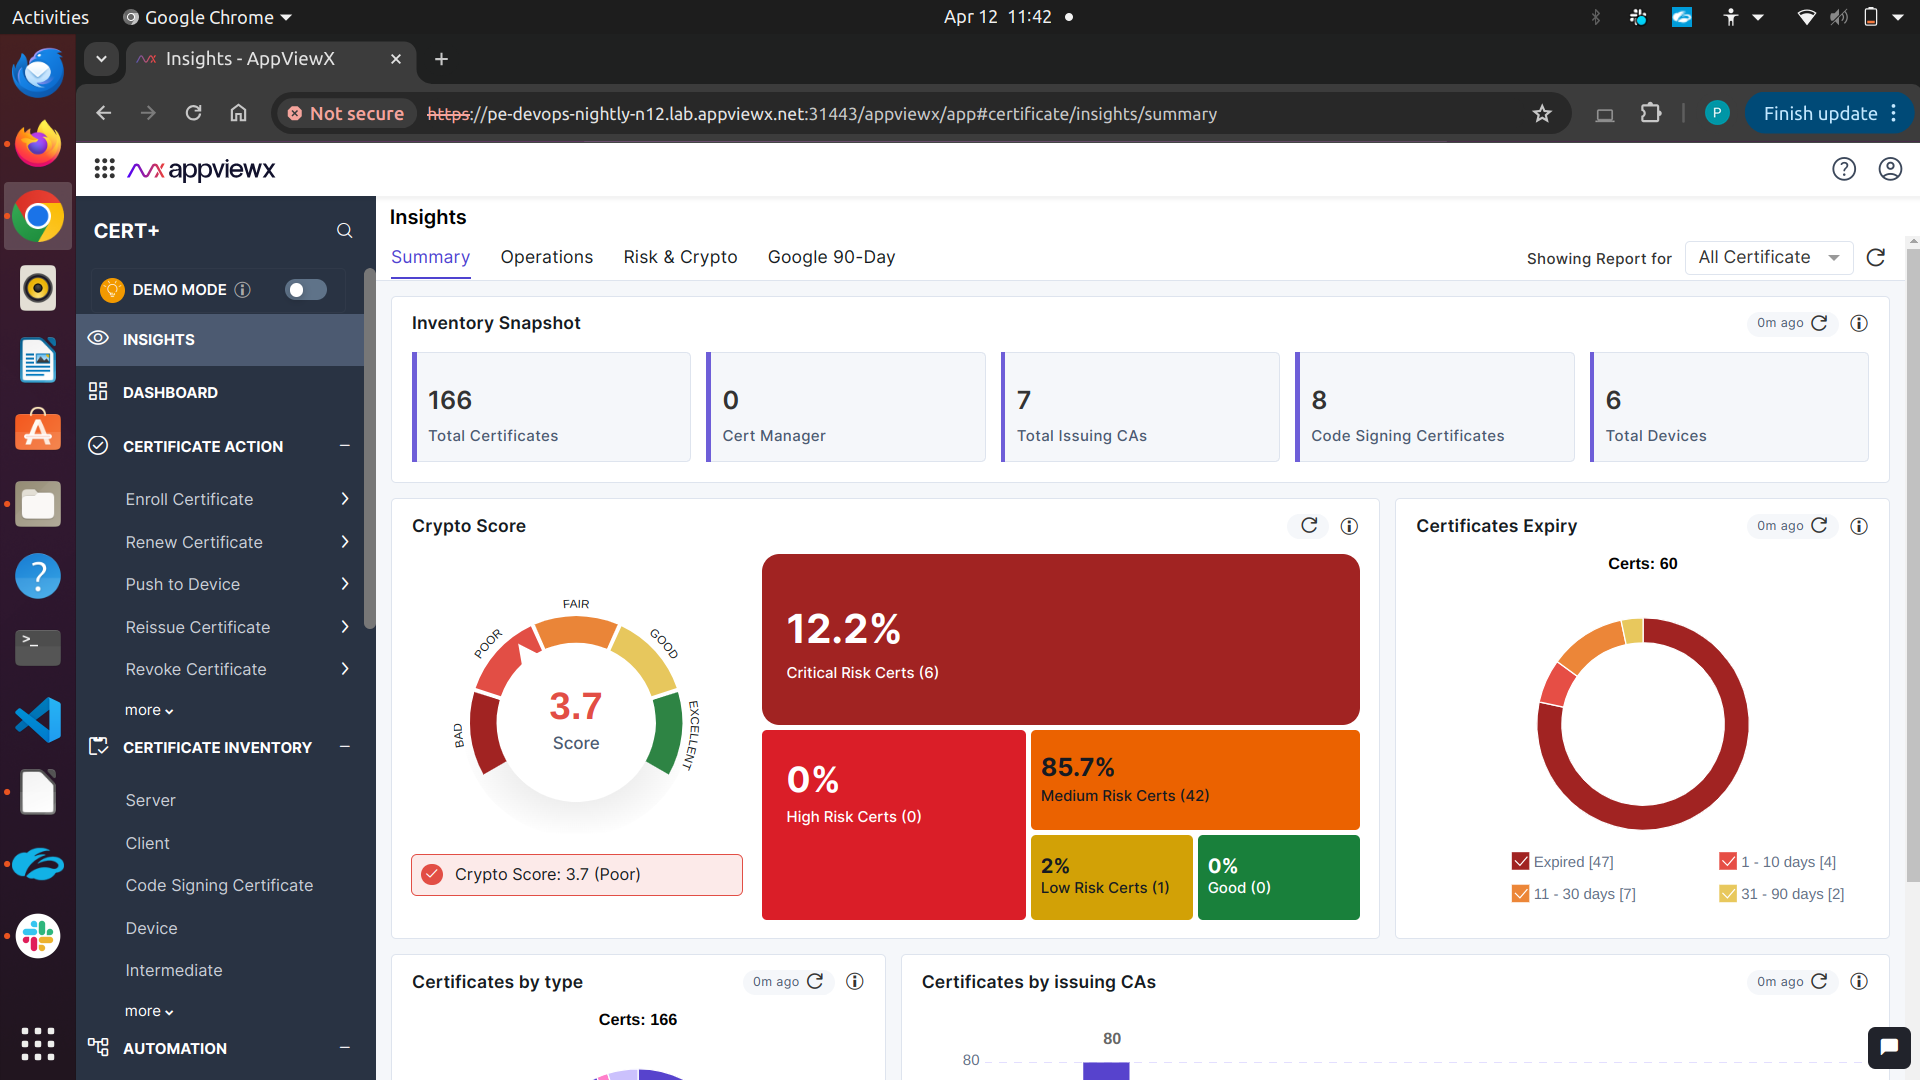
\includegraphics[width=0.8\textwidth]{dashboardStatics.png}
\caption{\textbf{Sample Result}}
\label{fig:sample_results}
\end{figure}

Attached is a sample result (Figure \ref{fig:sample_results}) showcasing the statistics of certificates.


\section{Sample Code}
\begin{lstlisting}
write your code here
main code
\end{lstlisting}
\subsubsection{Output}
\begin{figure}[H]
\centering
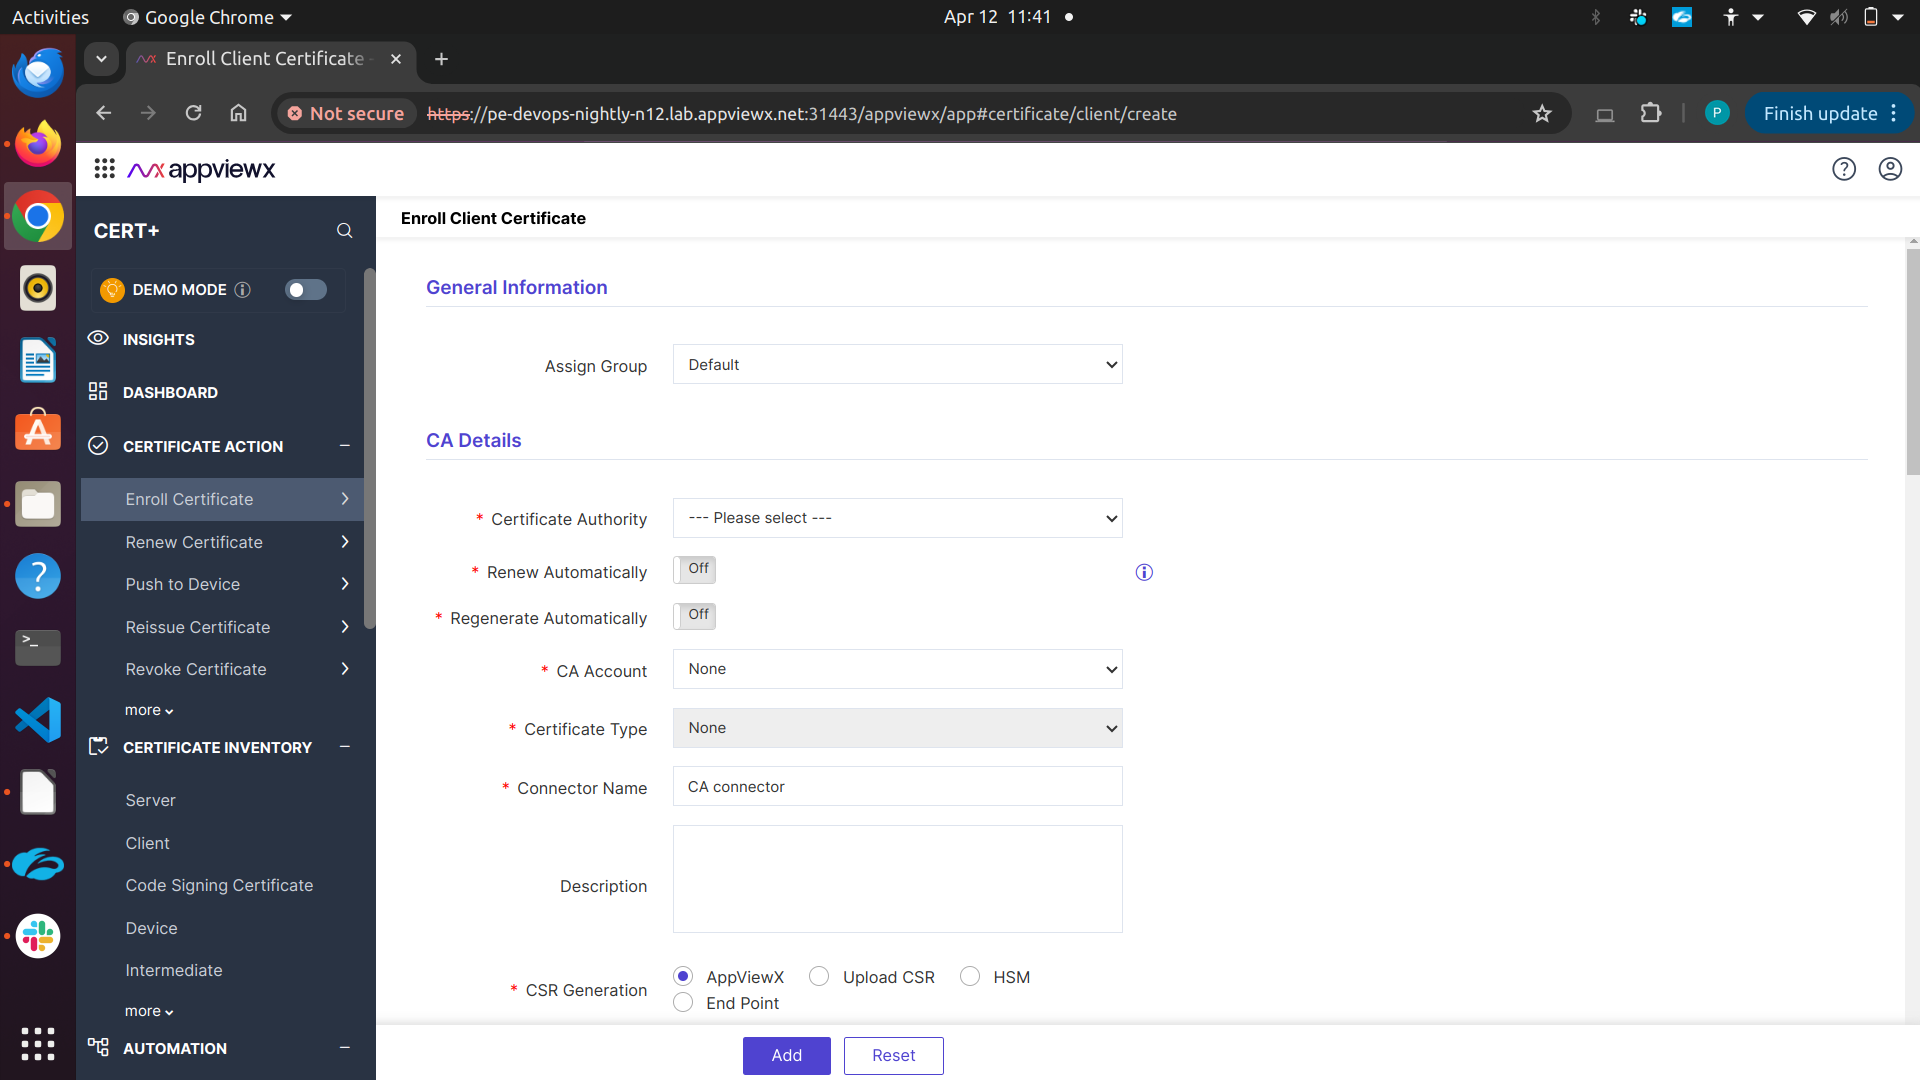
\includegraphics[height= 10cm, width=17cm]{certificateAction.png}
\caption{\textbf{Certificate Action}}
\end{figure}
\begin{figure}[H]
\centering
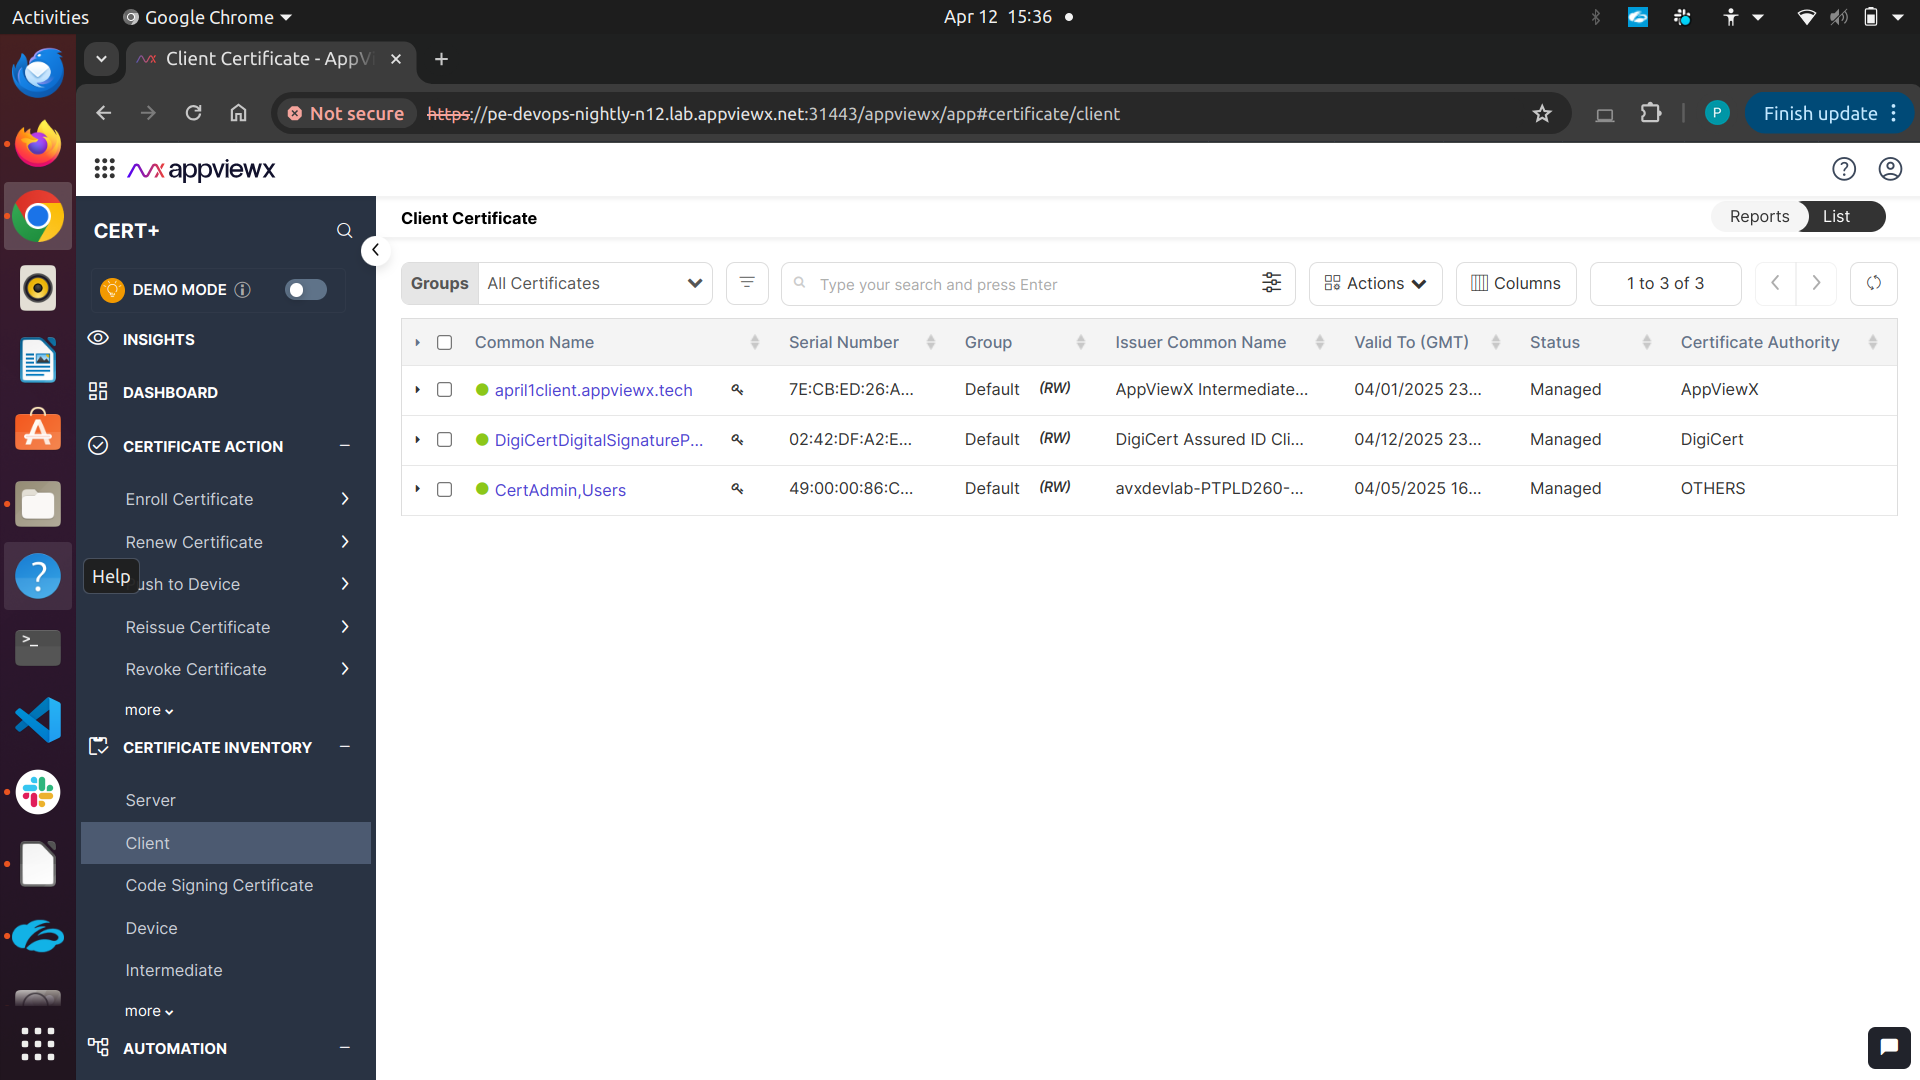
\includegraphics[height= 10cm, width=17cm]{certificateInventory.png}
\caption{\textbf{Certificate Inventory}}
\end{figure}

\begin{figure}[H]
\centering
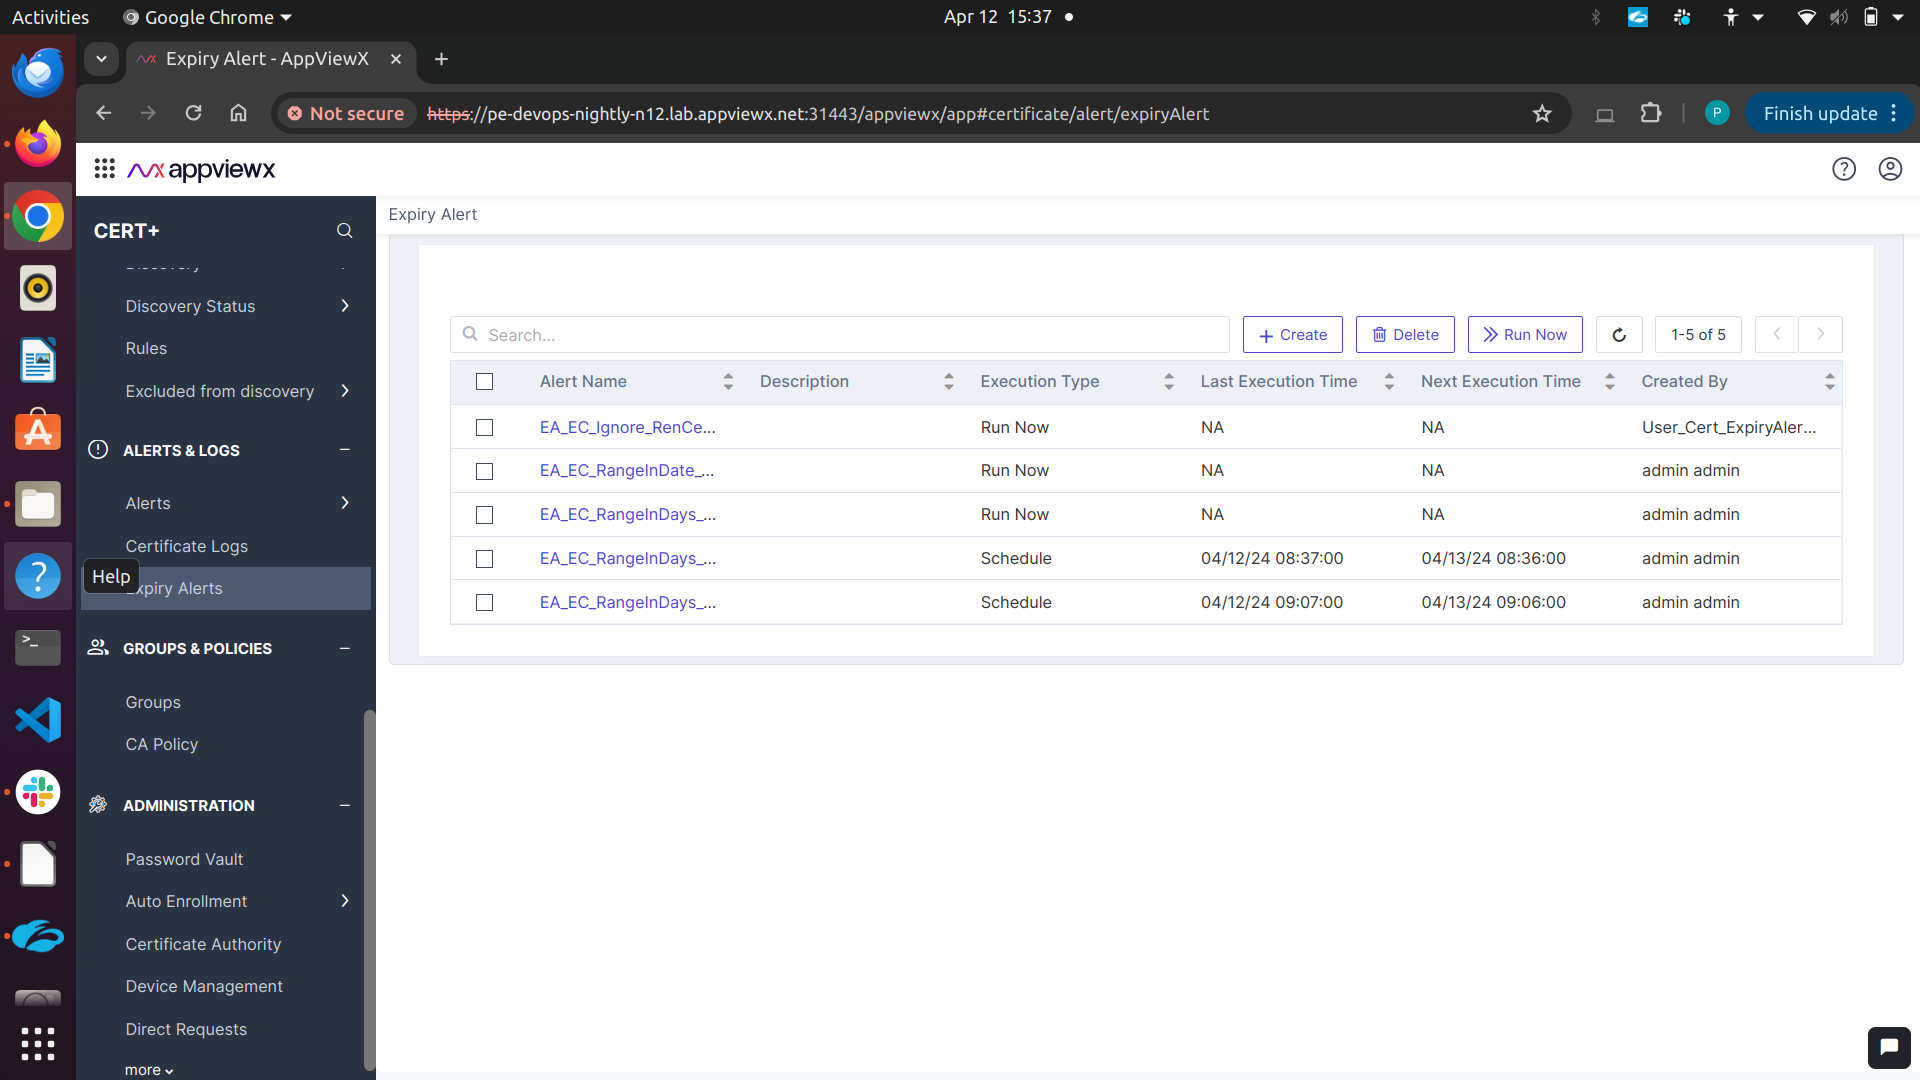
\includegraphics[height= 10cm, width=17cm]{expiryAlert.png}
\caption{\textbf{Expiry Alert}}
\end{figure}

\chapter{CONCLUSION AND FUTURE ENHANCEMENTS}
\linespread{1.5}
\section{Conclusion}
SHOULD BE MINIMUM TWO PARAGRAPHS -WITH MINIMUM 150 WORDS

\section{Future Enhancements}
SHOULD BE MINIMUM TWO PARAGRAPHS -WITH MINIMUM 150 WORDS
\chapter{INDUSTRY DETAILS}

\begin{itemize}
    \item Industry name: AppViewX
    \item Duration of Internship: (22/01/2024 - 22/07/2024)
    \item Duration of Internship in months: 6
    \item Industry Address: Module No: 107, 1st Floor, ELCOT SEZ, Tidel Park, Coimbatore, Tamil Nadu – 641014
    \item Internship offer letter:
    \href{https://drive.google.com/file/d/1si9CxusaIhOD625boEsVmmqiDDWzjc9q/view?usp=sharing} 
    \item Internship Completion certificate: Internship in Progress
    
\end{itemize}


\chapter{PLAGIARISM REPORT}
ATTACH ONLY SUMMARY PAGE OF PLAGIARISM REPORT

\chapter{SOURCE CODE \& POSTER PRESENTATION}
\section{Source Code}

\section{Poster Presentation}
Should be in New page after the source code

\addcontentsline{toc}{chapter}{References}
\renewcommand\bibname{References}

\begin{thebibliography}{9}
\bibitem {latexcompanion} \text{Pamella Soares; Raphael Saraiva; Iago Fernandes; Antônio Neto;
Jerffeson Souza(2022).A Blockchain-based Customizable Document Registration Service for Third
Parties, IEEE International Conference ,20(15),7456-7462}\\\\ \textbf{FORMAT:Author(s)name
(Year).Title, Journal name, Volume,
Issue, Pageno.}\\
\end{thebibliography}
\newpage

\begin{center} \textbf{General Instructions} \end{center}
\begin{itemize}
\item Cover Page should be printed as per the color template and the next page also should be
printed in color as per the template
\item \textbf {Wherever Figures applicable in Report , that page should be printed in color}
\item Dont include general content , write more technical content

\item Each chapter should minimum contain 3 pages
\item Draw the notation of diagrams properly

\item Every paragraph should be started with one tab space
\item Literature review should be properly cited and described with content related to project
\item All the diagrams should be properly described and dont include general information of any
diagram

\item Example Use case diagram - describe according to your project flow
\item All diagrams,figures should be numbered according to the chapter number and it should be
cited properly
\item\textbf {Testing and codequality should done in Sonarqube Tool}

\item Test cases should be written with test input and test output
\item All the references should be cited in the report
\item \textbf {AI Generated text will not be considered}

\item \textbf {Submission of Project Execution Files with Code in GitHub Repository}
\item \textbf {Thickness of Cover and Rear Page of Project report should be 180 GSM}
\item \textbf{Internship Offer letter and neccessary documents should be attached}
\item \textbf{Strictly dont change font style or font size of the template, and dont customize the
latex code of report}
\item \textbf{Report should be prepared according to the template only}
\item \textbf{Any deviations from the report template,will be summarily rejected}
\item \textbf{ Number of Project Soft Binded copy for each and every batch is (n+1) copies as given
in the table below}

\item For \textbf{Standards and Policies} refer the below link \\
https://law.resource.org/pub/in/manifest.in.html

\item Plagiarism should be less than 15\%
\item \textbf {Journal/Conference Publication proofs should be attached in the last page of Project
report after the references section}
\end{itemize}

\newpage

\includepdf[page=-]{Instructions-Major-intern}

\end{document}